\section{Malware Characteristics}

\subsection{General characteristics}

We observe three characteristics after analyzing data we collect:

{\bf Observation 1:} 
most malwares are submitted only once to VirusTotal. 
We have collected 4732502 PE malware submissions, and there are in total 4038647 distinct PE malwares. 
On average, each PE malware is submitted 1.17 times to VirusTotal. 
We believe that most malwares are encountered by more than one VirusTotal user. 
We think this observation is likely to be caused by the fact that VirusTotal users 
tend to check whether their samples have already been submitted, 
before conducting their submissions, 
and the number of submissions is not a good indicator for malware popularity. 


{\bf Observation 2:} 
100 - 400 new malware families would appear each day. 
Figure~\ref{fig:new} shows new malwares appeared in November of 2015. 
We do not have any data before Nov. 1st, 
so there are much more new malware families in the first few days.
After that, the number of new malware families is roughly from 100 to 400. 
In total, there are 11311 malware families. 




\begin{figure}[t!]
\begin{center}
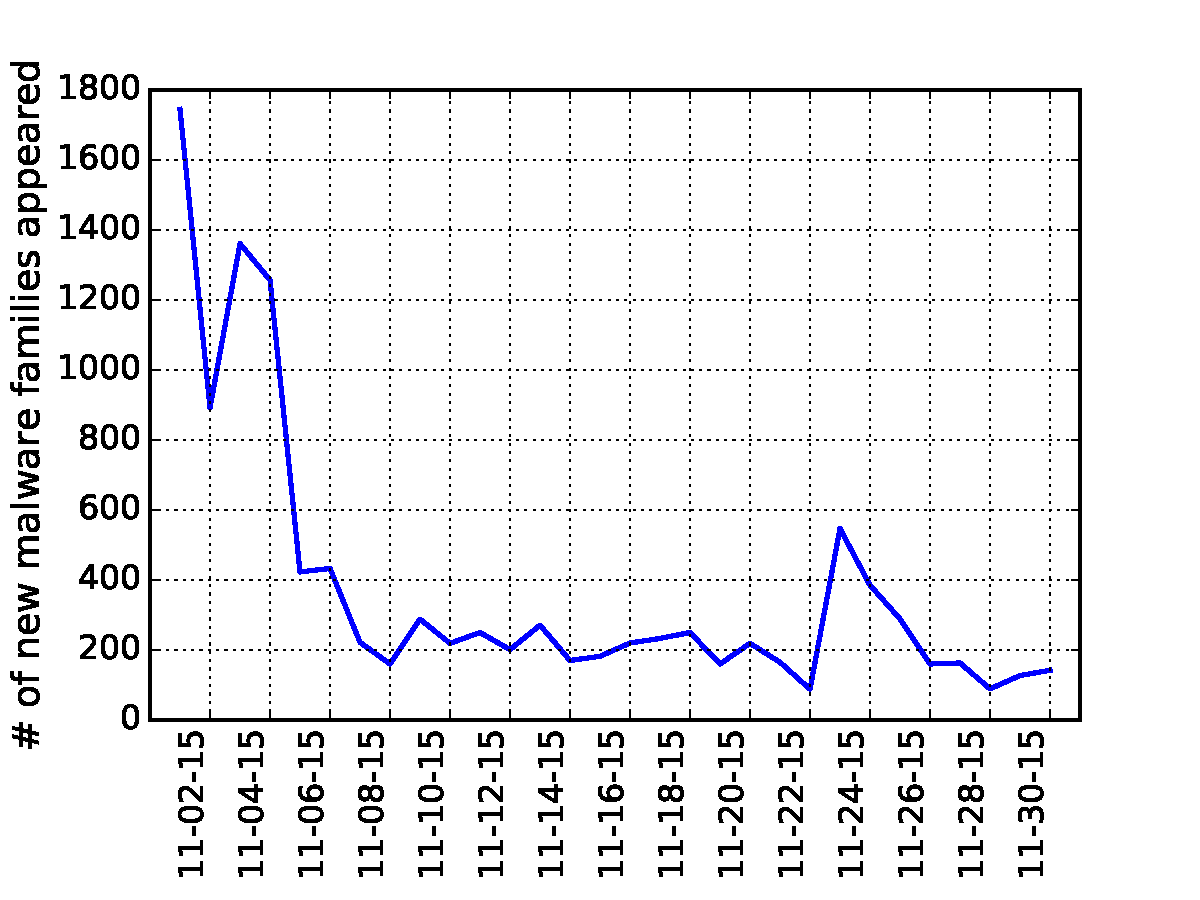
\includegraphics[width=3.0in]{figure/new_family}
\caption{The number of new malware families we observed each day in November of 2015.}
\label{fig:new}
\end{center}
\end{figure}

\begin{figure}[t!]
\begin{center}
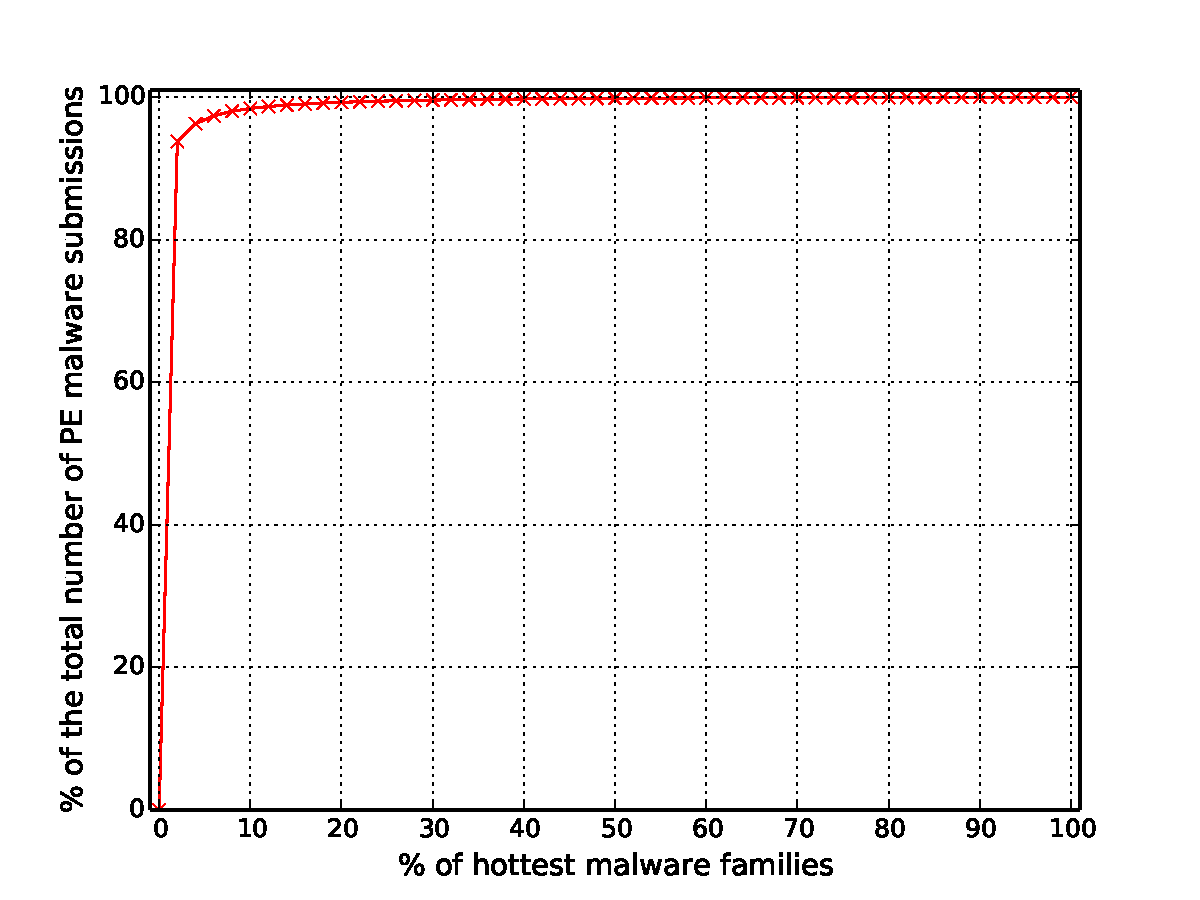
\includegraphics[width=3.0in]{figure/cum}
\caption{Skewness of malware families appearing in November of 2015.}
\label{fig:acum}
\end{center}
\end{figure}

{\bf Observation 3:} 
The distribution of malware families are highly skewed. 
As shown in Figure~\ref{fig:acum}, only small number of malware families are hot.
The distribution of malware families follows the well-known Pareto principle, 
and more than 90\% malware families take place in only 10\% malwares. 
The skewness of malware family distribution suggests that we could conduct effective hot malware family mining. 


\subsection{Temporal Characteristics}
\label{sec:predict}

%\subsection{Overview}

\begin{figure}[t!]
\begin{center}
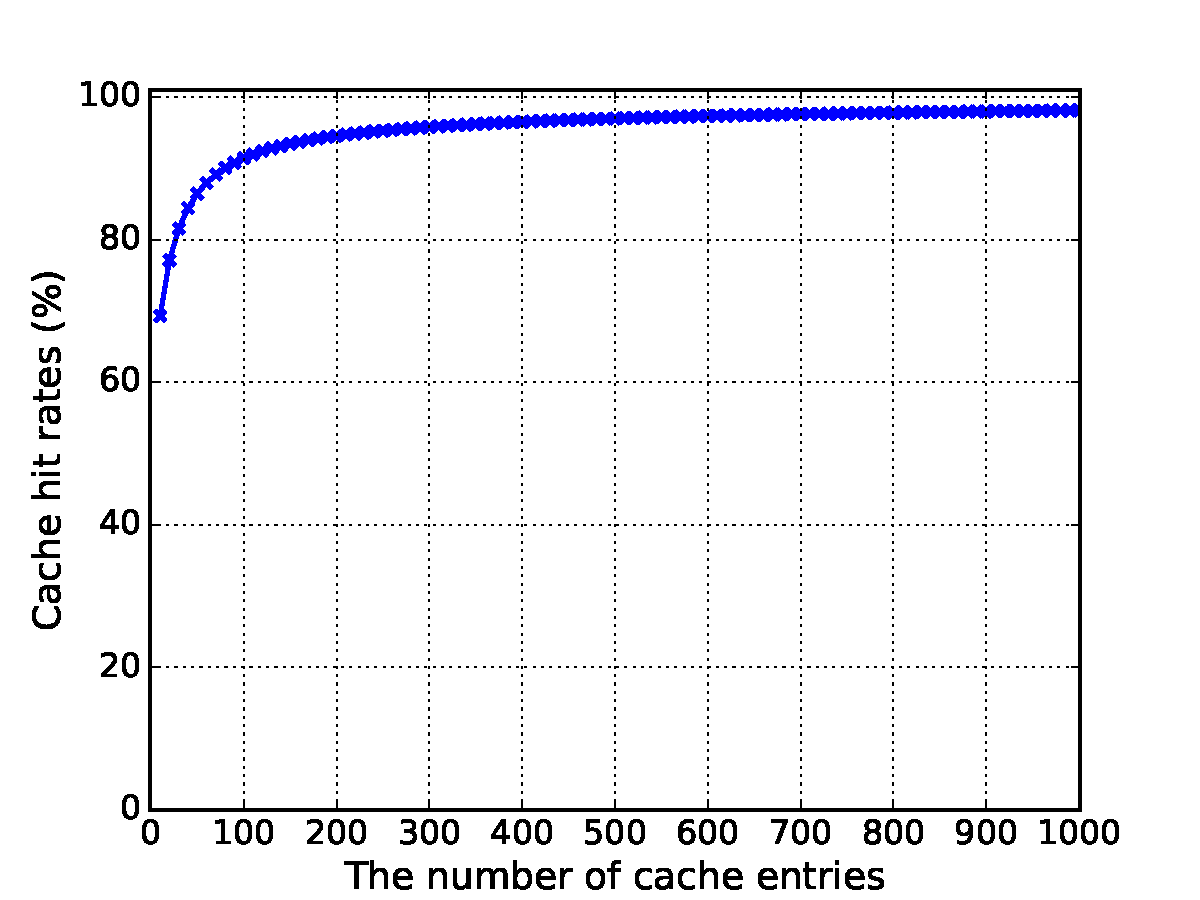
\includegraphics[width=3.0in]{figure/LRU}
\caption{Relation between cache hit rate and cache size.}
\label{fig:cache}
\end{center}
\end{figure}


\begin{figure}[t!]
\begin{center}
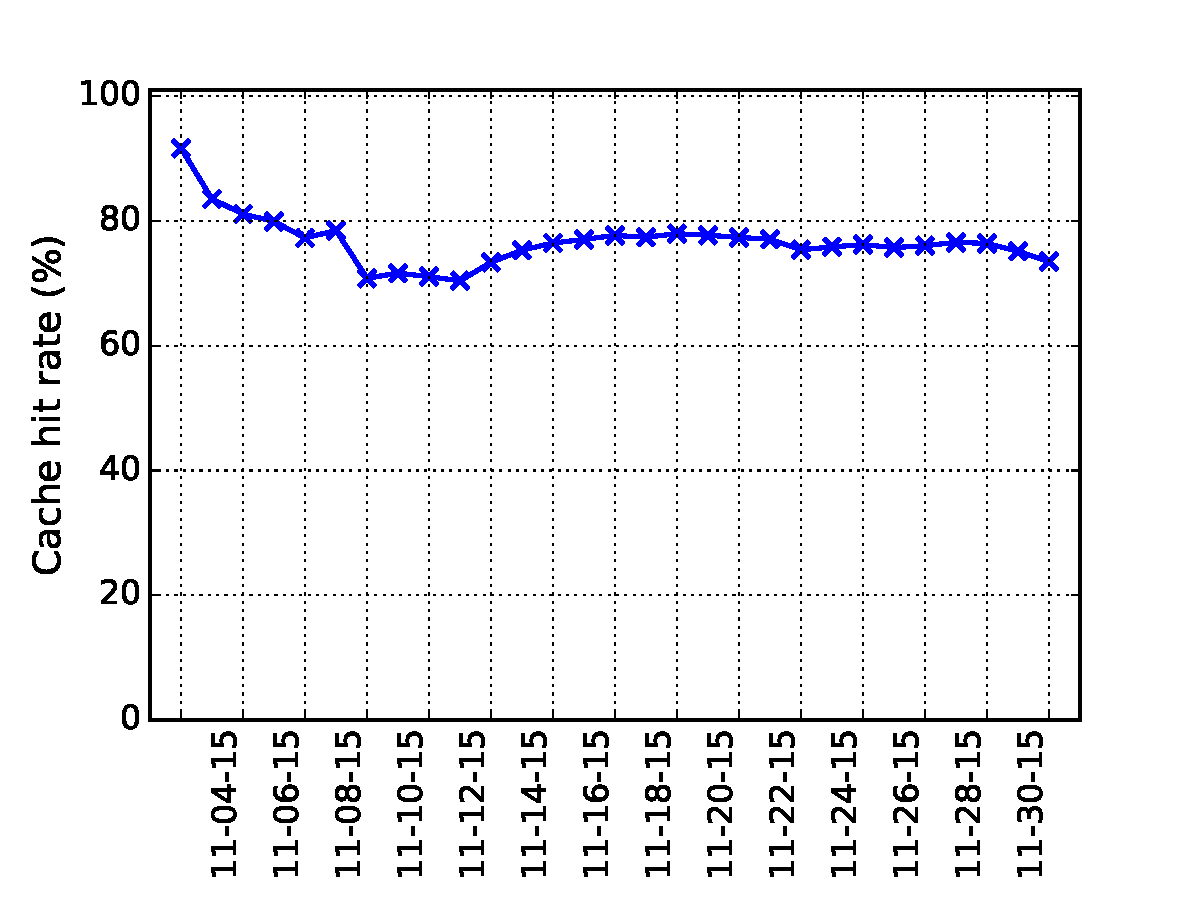
\includegraphics[width=3.0in]{figure/LRU_day}
\caption{Cache hit rate during per-day update.}
\label{fig:batchcache}
\end{center}
\end{figure}

Resources to combat malwares are limited. 
Any techniques that could allow antivirus vendors to focus their effort would be great. 
In this section, we build a solution, which can predict malwares belonging to which families would appear in the near future. 
The basic intuition behind our technique is that malwares do not appear uniformly across different family and time, but they appear in bursts.
We borrow cache mechanism from system areas to conduct our prediction. 

There are several notions in cache terminology: 
block size is defined as how many entries would be added into cache or evicted from cache together.
Pre-fetch means loading entries that cache has not encountered yet. 
Replacement policy control how to evict entries from cache, when the cache is full. 
We use the most preliminary cache setting. We fix the block size to be 1, disable pre-fetch, 
and use LRU (least recently used) replacement policy. We use N to represent the cache size
Our malware family cache works as follows:  

We start with empty cache. 
For a new malware submission, if the malware family is already in cache, we will move the cache entry to the front our cache entry list. 
If the new malware family is not in cache, 
we will create a new cache entry, and add it into the front of our cache entry list. 
If cache is full, we need to evict the entry at the end. 


%\subsection{Evaluation}

We implement our cache by using python-2.7, 
and conduct the experiment on the same machine as in Section~\ref{sec:eval1}. 
We measure hit rate to evaluate our solution, and hit rate is calculated as: 

$$ \mbox{hit rate} = \dfrac{\mbox{\# of hits}}{\mbox{\# of hits + \# of misses}}$$

We conduct two experiments. In the first experiment, 
we explore how cache hit rate changes with the number of cache entries. 
We change cache size from 10 to 1000. As shown in Figure~\ref{fig:cache}, 
the rate rate will grow from 69.29\% to 98.14\%. 
By using more than 80 cache entries, the cache hit rate will be above 90\%, 
and by using more than 230 cache entries, the cache hit rate will be above 95\%. 

In the second experiment, we fix the cache size to 100, 
and we use the cache content got from previous day to calculate cache hit rate, 
and only update cache content at the end of each day. Figure~\ref{fig:batchcache} show the cache hit rate each day. 
Most cache hit rate falls between 70\% and 80\%.  

%\subsection{Discussion}
There are many other cache block size, pre-fetch mechanism, and replacement policy proposed in previous works. 
We leave explore the effect of their combinations in the future. 
As we discussed in Section~\ref{sec:discussion1}, 
we could also explore how to change the prediction granularity from malware family to ssdeep-based clusters. 
